%%%%%%%%%%%%%%%%%%%%%%%%%%%%%%%%%%%%%%%%%
% Beamer Presentation
% LaTeX Template
% Version 1.0 (10/11/12)
%
% This template has been downloaded from:
% http://www.LaTeXTemplates.com
%
% License:
% CC BY-NC-SA 3.0 (http://creativecommons.org/licenses/by-nc-sa/3.0/)
%
%%%%%%%%%%%%%%%%%%%%%%%%%%%%%%%%%%%%%%%%%

%----------------------------------------------------------------------------------------
%	PACKAGES AND THEMES
%----------------------------------------------------------------------------------------

\documentclass{beamer}

\mode<presentation> {

% The Beamer class comes with a number of default slide themes
% which change the colors and layouts of slides. Below this is a list
% of all the themes, uncomment each in turn to see what they look like.

%\usetheme{default}
%\usetheme{AnnArbor}
%\usetheme{Antibes}
%\usetheme{Bergen}
%\usetheme{Berkeley}
%\usetheme{Berlin}
%\usetheme{Boadilla}
%\usetheme{CambridgeUS}
%\usetheme{Copenhagen}
%\usetheme{Darmstadt}
%\usetheme{Dresden}
%\usetheme{Frankfurt}
%\usetheme{Goettingen}
%\usetheme{Hannover}
%\usetheme{Ilmenau}
%\usetheme{JuanLesPins}
%\usetheme{Luebeck}
%\usetheme{Madrid}
%\usetheme{Malmoe}
%\usetheme{Marburg}
%\usetheme{Montpellier}
\usetheme{PaloAlto}
%\usetheme{Pittsburgh}
%\usetheme{Rochester}
%\usetheme{Singapore}
%\usetheme{Szeged}
%\usetheme{Warsaw}

% As well as themes, the Beamer class has a number of color themes
% for any slide theme. Uncomment each of these in turn to see how it
% changes the colors of your current slide theme.

%\usecolortheme{albatross}
%\usecolortheme{beaver}
%\usecolortheme{beetle}
%\usecolortheme{crane}
%\usecolortheme{dolphin}
%\usecolortheme{dove}
%\usecolortheme{fly}
%\usecolortheme{lily}
%\usecolortheme{orchid}
%\usecolortheme{rose}
%\usecolortheme{seagull}
\usecolortheme{seahorse}
%\usecolortheme{whale}
%\usecolortheme{wolverine}

%\setbeamertemplate{footline} % To remove the footer line in all slides uncomment this line
%\setbeamertemplate{footline}[page number] % To replace the footer line in all slides with a simple slide count uncomment this line

%\setbeamertemplate{navigation symbols}{} % To remove the navigation symbols from the bottom of all slides uncomment this line
}
\def\insertlogoright{\usebeamertemplate*{logoright}}
\def\logoright{\setbeamertemplate{logoright}}
\makeatletter
  \defbeamertemplate*{headline}{mycustom theme}
  {%
    \begin{beamercolorbox}[wd=\paperwidth]{frametitle}
      \ifx\beamer@sidebarside\beamer@lefttext%
      \else%
        \hfill%
      \fi%
      \ifdim\beamer@sidebarwidth>0pt%  
        \usebeamercolor[bg]{logo}%
        \vrule width\beamer@sidebarwidth height \beamer@headheight%
        \hskip-\beamer@sidebarwidth%
        \hbox to \beamer@sidebarwidth{%
        \hss%
        \vbox to \beamer@headheight{%
        \vss\hbox{\color{fg}\insertlogo}\vss%
        }%
        \hss}%
        \hfill%
        \hbox to \beamer@sidebarwidth{%
        \hss%
        \vbox to \beamer@headheight{%
        \vss\hbox{\color{fg}\insertlogoright}\vss%
        }%
        \hss}%
      \else%
        \vrule width0pt height \beamer@headheight%  
      \fi%
    \end{beamercolorbox}
  }
\makeatother

\setbeamercovered{transparent}
\languagepath{spanish}
\usepackage{graphicx} % Allows including images
\usepackage{booktabs} % Allows the use of \toprule, \midrule and \bottomrule in tables
\usepackage[spanish]{babel}
\usepackage[utf8]{inputenc}
%----------------------------------------------------------------------------------------
%	TITLE PAGE
%----------------------------------------------------------------------------------------
\logo{
\includegraphics[height=1.5cm]{img/logo_uach.png}}
\logoright{
\includegraphics[width=2.3cm,keepaspectratio]{img/alta-color-60x30.png}\hspace{50pt}}
\title[Proyecto de Tesis]{Sistema de apoyo al monitoreo curricular de Estudios de pregrado UACh} % The short title appears at the bottom of every slide, the full title is only on the title page

\author{Baldomero Águila Napoli} % Your name
\institute[UACh] % Your institution as it will appear on the bottom of every slide, may be shorthand to save space
{
Universidad Austral de Chile \\ % Your institution for the title page
\medskip
\textit{Patrocinante: Mauricio Ruiz-Tagle} % Your email address
}
\date{\today} % Date, can be changed to a custom date

\begin{document}

\begin{frame}
\titlepage % Print the title page as the first slide
\end{frame}

\begin{frame}
\frametitle{Contenidos} % Table of contents slide, comment this block out to remove it
\tableofcontents[pausesections] % Throughout your presentation, if you choose to use \section{} and \subsection{} commands, these will automatically be printed on this slide as an overview of your presentation
\end{frame}

%----------------------------------------------------------------------------------------
%	PRESENTATION SLIDES
%----------------------------------------------------------------------------------------

%------------------------------------------------
\section{Introducción} % Sections can be created in order to organize your presentation into discrete blocks, all sections and subsections are automatically printed in the table of contents as an overview of the talk
%------------------------------------------------

\begin{frame}
\frametitle{Introducción}
\framesubtitle{Modelo  educacional de la Universidad Austral de Chile}
\begin{figure}
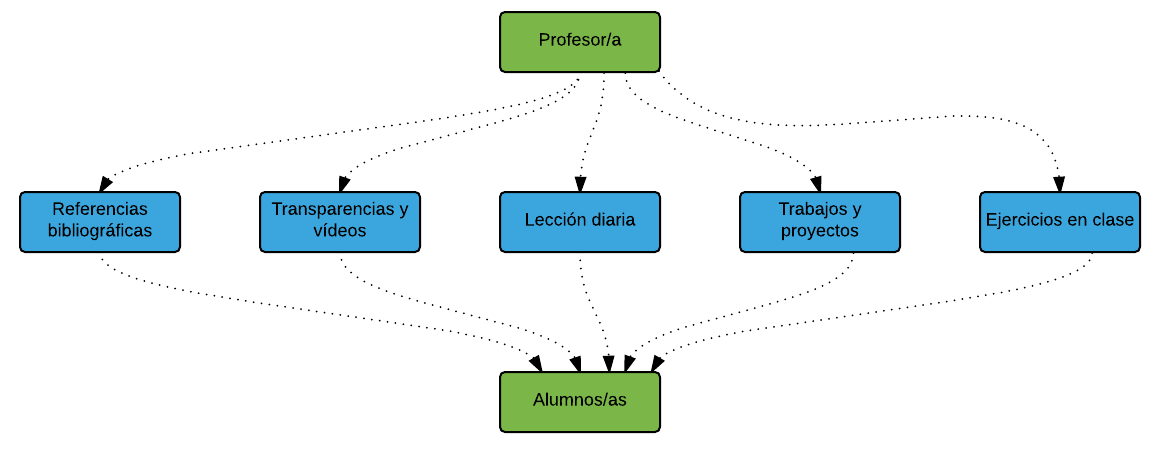
\includegraphics[height=4.2cm]{img/modelo_centrado_ensenianza.png}
\caption{Enfoque educacional tradicional.}
\end{figure}
\end{frame}

%------------------------------------------------

\begin{frame}
\frametitle{Introducción}
\framesubtitle{Innovación curricular}
\begin{figure}
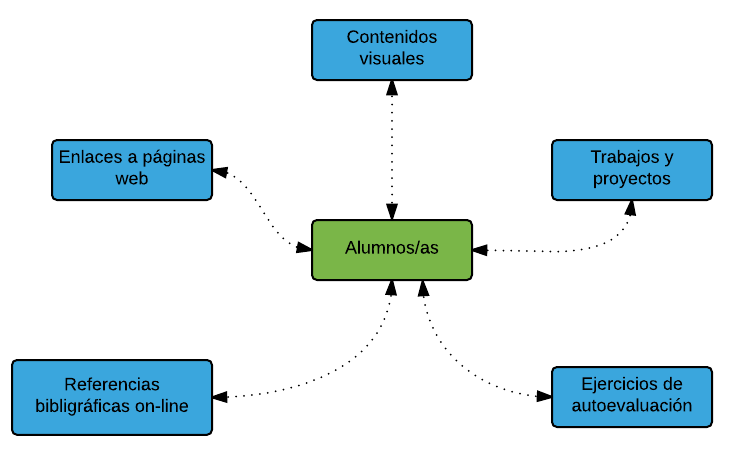
\includegraphics[height=6cm]{img/modelo_centrado_alumno.png}
\caption{Enfoque educacional centrado en el estudiante.}
\end{figure}
\end{frame}

%------------------------------------------------





\begin{frame}
\frametitle{Introducción}
\framesubtitle{Departamentos que realizan la Innovación curricular en la UACh}

\begin{itemize}
	\item Departamento de Aseguramiento de la Calidad e innovación Curricular.
	\begin{itemize}
		\item Apoyo al Desarrollo y la Innovación Curricular en Pregrado.
	\end{itemize}
	\item Departamento de Admisión y Matrícula.
	\item Departamento de Registro Académico Estudiantil.

\end{itemize}
\end{frame}

%------------------------------------------------



\begin{frame}  
\frametitle{Introducción}     
    \framesubtitle{Modificación curricular mayor y/o menor}
	\framezoom<1><2>(1cm,0cm)(4cm,2.3cm)
	\framezoom<1><3>[border](3.5cm,1cm)(2cm,3cm)
	\framezoom<1><4>(4cm,3cm)(5.3cm,3cm) % mover (xarriba abajo,izquierda derecha)  luego tamaño x,y

    
    \begin{figure}
        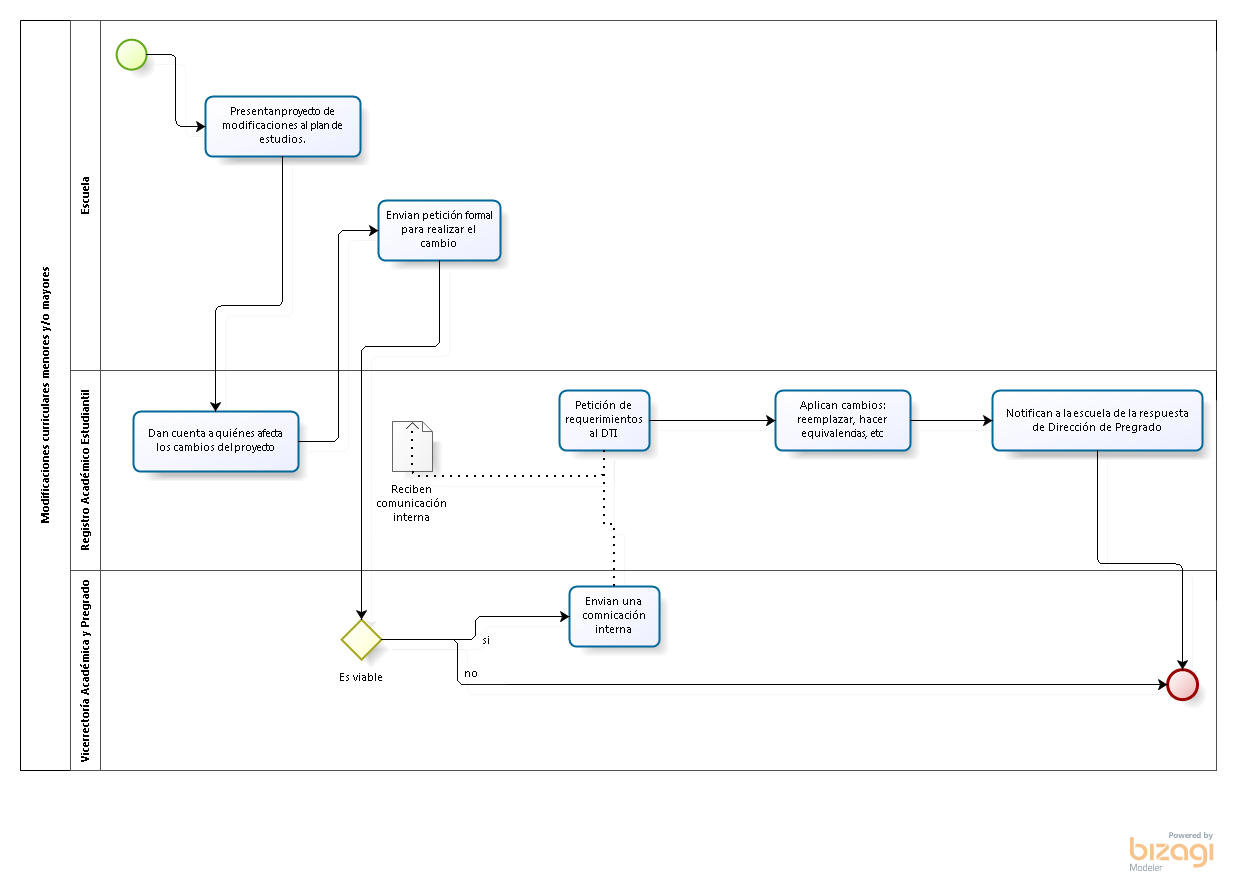
\includegraphics[height=6cm]{img/Procesos_cambios_curriculares.png}
        \caption{Diagrama de procesos de los cambios curriculares Mayores y Menores.}
    \end{figure}        
\end{frame} 

%------------------------------------------------
\begin{frame}    
\frametitle{Introducción}   
    \framesubtitle{Creación de nuevas carreras}
	\framezoom<1><2>(0.9cm,0.3cm)(2cm,2cm)
	\framezoom<1><3>(0.9cm,2.9cm)(7cm,2cm)
	\framezoom<1><4>(5cm,1cm)(5cm,3cm)
    
    \begin{figure}
        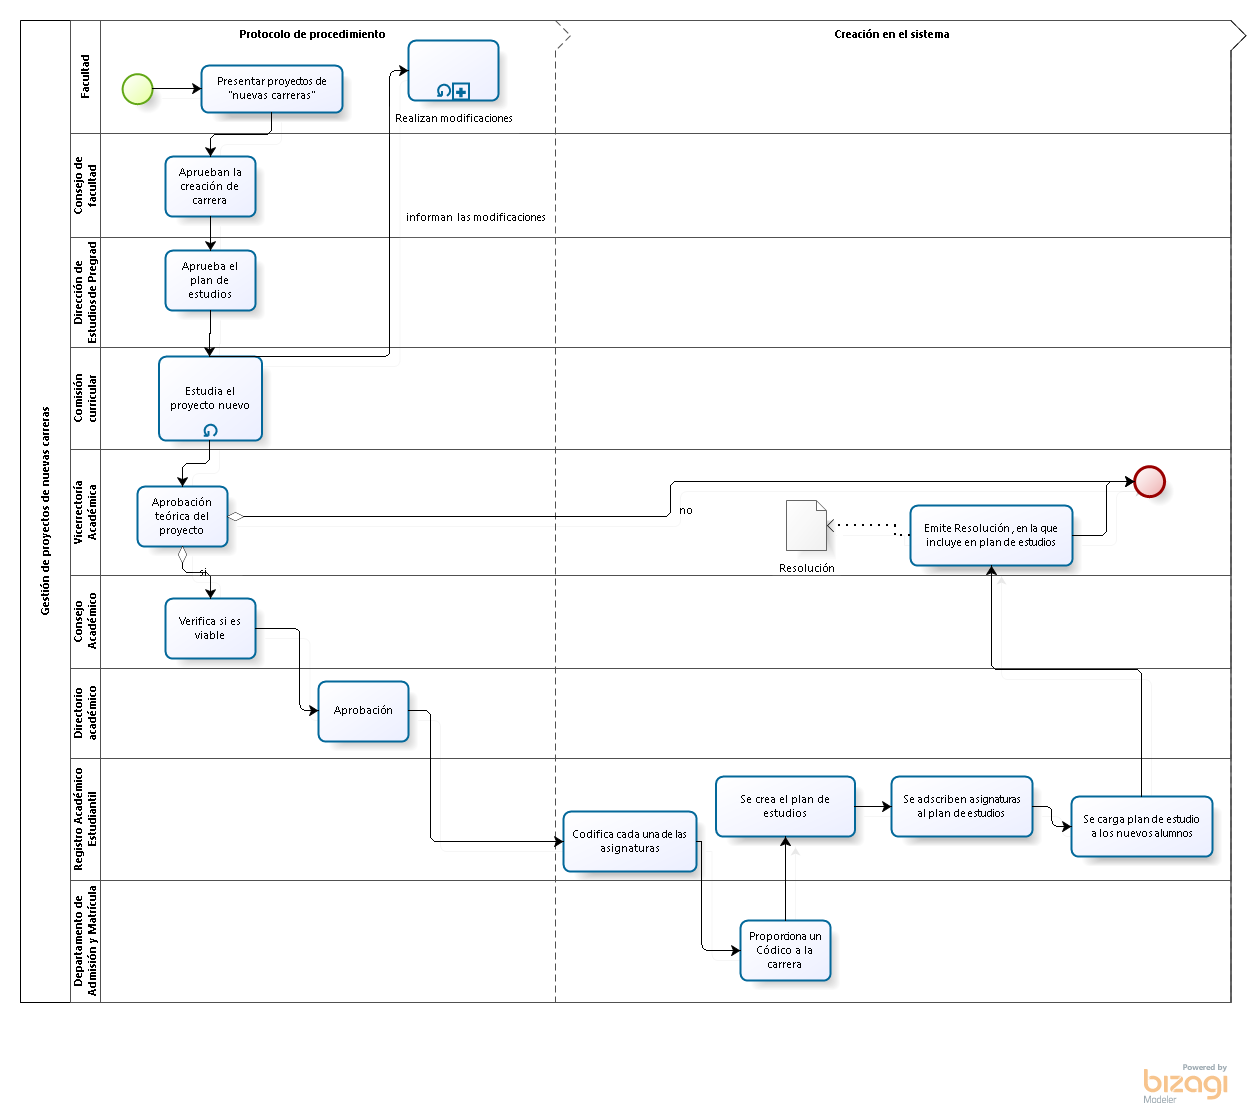
\includegraphics[height=6cm]{img/Procesos_Registro_academico.png}
        \caption{Diagrama de procesos de creación de nuevas carreras.}
    \end{figure}        
\end{frame} 

%------------------------------------------------

\begin{frame}
\frametitle{Introducción}
\framesubtitle{Documentos con los que trabaja Dirección de Estudios de Pregrado}
\begin{block}{Documentos}
\begin{itemize}
	\item Comunicación interna.
	\item Correos electrónicos.
	\item Resolución.
	\item Decretos.
\end{itemize}
\end{block}
\end{frame}
%------------------------------------------------
\begin{frame}    
\frametitle{Introducción}   
    \framesubtitle{Principal problema}

    
    \begin{figure}
        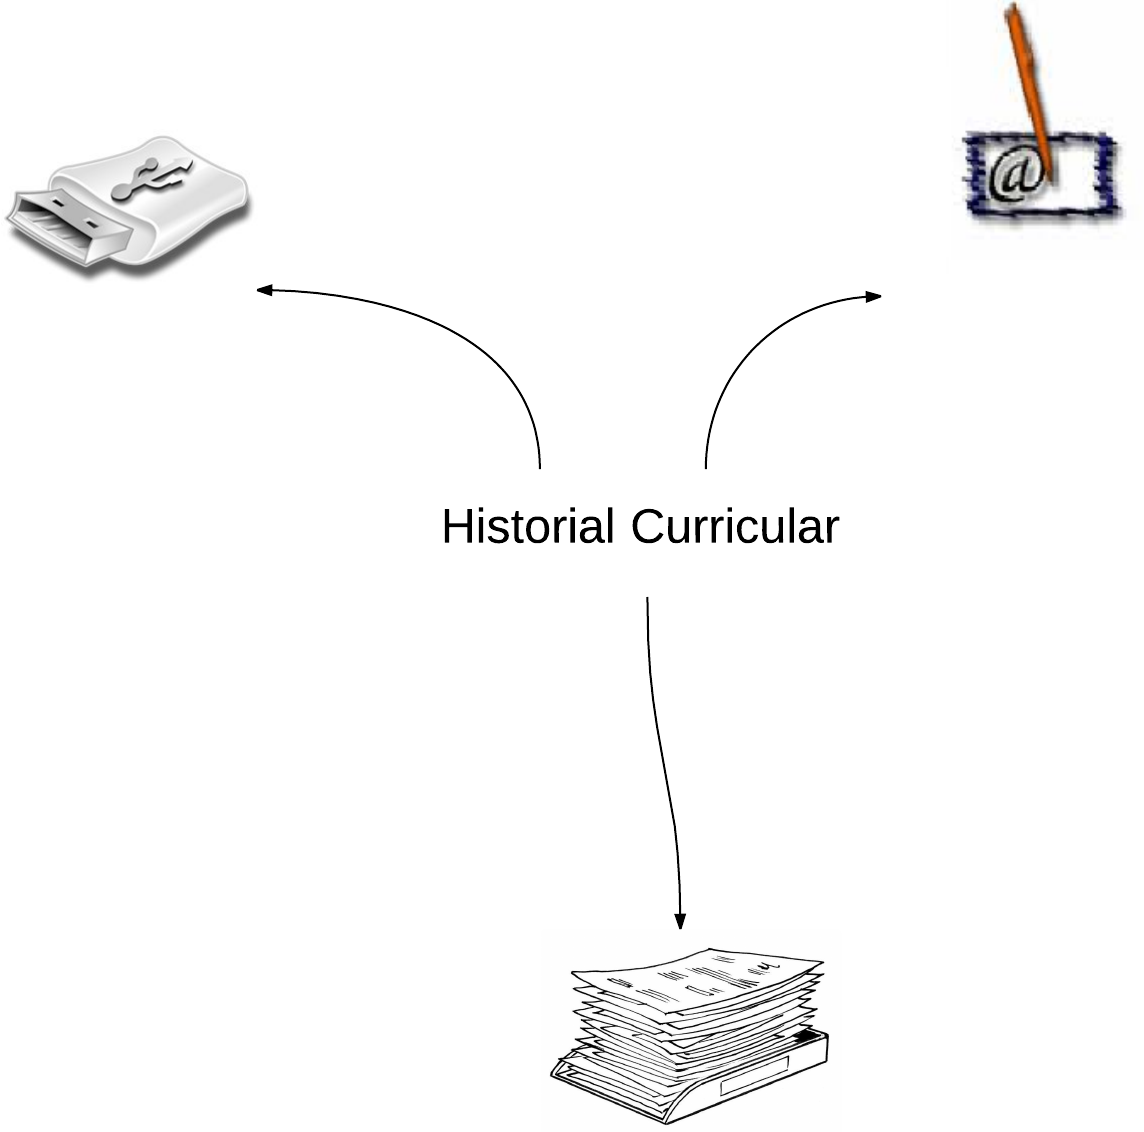
\includegraphics[height=6cm]{img/intento_numero_1000.png}
        \caption{Medios de almacenamiento.}
    \end{figure}        
\end{frame} 




%------------------------------------------------


\begin{frame}
\frametitle{Introducción}
\framesubtitle{Objetivo general}
\pause
\begin{block}{Objetivo general}
	Diseñar y construir  un prototipo de una plataforma web que apoye al monitoreo curricular de pregrado.
\end{block}
\end{frame}

%------------------------------------------------






%------------------------------------------------
\section{Marco teórico}
%------------------------------------------------

\begin{frame}
\frametitle{Marco teórico}
\framesubtitle{Pseudo MVC}
    \begin{figure}
        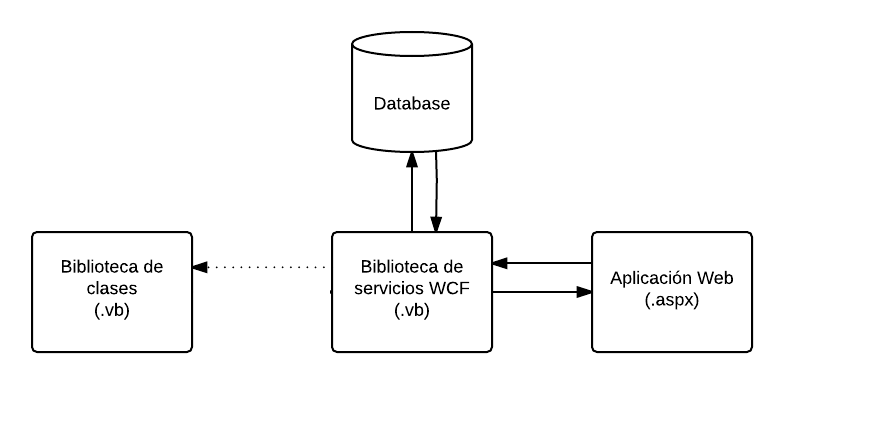
\includegraphics[height=6cm]{img/pseudoMVC.png}
        \caption{Arquitectura MVC de la Universidad Austral de Chile}
    \end{figure}  
\end{frame}
%------------------------------------------------

\begin{frame}
\frametitle{Marco teórico}
\framesubtitle{Tecnologías}
\pause
\begin{block}{Frond-End}
\begin{itemize}
	\item Jquery.
	\item Alertify.
	\item Bootstrap.
	\item 	Template Metis.
	\item Parsley.
\end{itemize}
\end{block}
\pause
\begin{block}{Back-End}
\begin{itemize}
	\item Microsoft SQL Server 2008.
	\item ASP.NET.
\end{itemize}
\end{block}
\end{frame}



%------------------------------------------------
\section{Desarrollo}
%------------------------------------------------
\begin{frame}
\frametitle{Desarrollo}
\framesubtitle{Metodología}

    \begin{figure}
        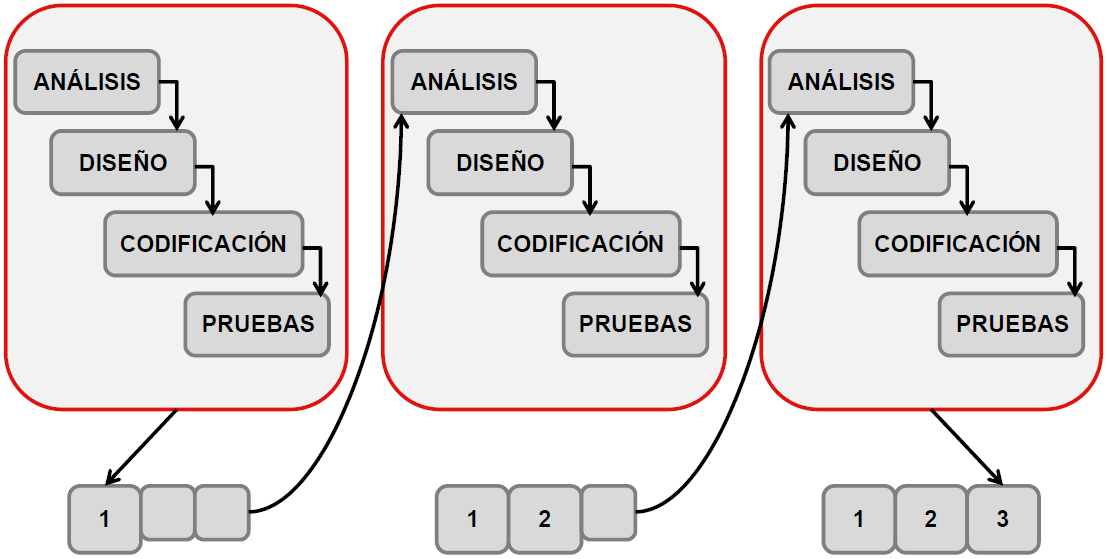
\includegraphics[height=4cm]{img/INCREMENTAL.png}
        \caption{Ciclo de vida incremental}
    \end{figure} 
   	\begin{itemize}[<+->]
   	
		\item Incremento 1: Historial curricular.
		\item Incremento 2: Gestión de documentos.
		\item Incremento 3: Gestión de usuarios.
	\end{itemize} 
\end{frame}

%------------------------------------------------
\begin{frame}
\frametitle{Desarrollo}
\framesubtitle{Requerimientos}

    \begin{block}{Requerimientos funcionales}
    	\begin{itemize}
    		\item<1-> Autentificación de usuario.
    		\item<2-> Gestión de perfil.
    		\item<3-|alert@10> Desplegar historial curricular.
    		\item<4-> Registro de usuarios.
    		\item<5-|alert@10> Gestión de documentos.
    		\item<6-> Visor de PDF.
    		\item<7-> Notificaciones.
    		\item<8-> Almacenar bitácora de los usuarios.
    		\item<9-> Visualización de la bitácora.
    		
    	\end{itemize}
	\end{block}     
\end{frame}

%------------------------------------------------
\begin{frame}
\frametitle{Desarrollo}
\framesubtitle{Requerimientos}

    \begin{block}{Requerimientos no  funcionales}
    	\begin{itemize}
    		\item<1-> Ambiente web.
    		\item<2-> Escalabilidad.
    		\item<3-> Fácil de usar.
    		\item<4-> Facilidad de pruebas.
    		\item<5-> Reglas de validación.
    		\item<6-> Acoplación.
    		
    	\end{itemize}
	\end{block}     
\end{frame}



%------------------------------------------------
\subsection{Requerimientos funcionales} 
\begin{frame}
\frametitle{Table}
\begin{table}
\begin{tabular}{l l l}
\toprule
\textbf{Treatments} & \textbf{Response 1} & \textbf{Response 2}\\
\midrule
Treatment 1 & 0.0003262 & 0.562 \\
Treatment 2 & 0.0015681 & 0.910 \\
Treatment 3 & 0.0009271 & 0.296 \\
\bottomrule
\end{tabular}
\caption{Table caption}
\end{table}
\end{frame}

%------------------------------------------------
\subsection{requerimientos no funcionales} 
\begin{frame}
\frametitle{Table}
\begin{table}
\begin{tabular}{l l l}
\toprule
\textbf{Treatments} & \textbf{Response 1} & \textbf{Response 2}\\
\midrule
Treatment 1 & 0.0003262 & 0.562 \\
Treatment 2 & 0.0015681 & 0.910 \\
Treatment 3 & 0.0009271 & 0.296 \\
\bottomrule
\end{tabular}
\caption{Table caption}
\end{table}
\end{frame}
%------------------------------------------------
\subsection{Modelo Conceptual} 
\begin{frame}
\frametitle{Table}
\begin{table}
\begin{tabular}{l l l}
\toprule
\textbf{Treatments} & \textbf{Response 1} & \textbf{Response 2}\\
\midrule
Treatment 1 & 0.0003262 & 0.562 \\
Treatment 2 & 0.0015681 & 0.910 \\
Treatment 3 & 0.0009271 & 0.296 \\
\bottomrule
\end{tabular}
\caption{Table caption}
\end{table}
\end{frame}
%------------------------------------------------


\subsection{Modelo de datos} 
\begin{frame}
\frametitle{Table}
\begin{table}
\begin{tabular}{l l l}
\toprule
\textbf{Treatments} & \textbf{Response 1} & \textbf{Response 2}\\
\midrule
Treatment 1 & 0.0003262 & 0.562 \\
Treatment 2 & 0.0015681 & 0.910 \\
Treatment 3 & 0.0009271 & 0.296 \\
\bottomrule
\end{tabular}
\caption{Table caption}
\end{table}
\end{frame}
%------------------------------------------------

\subsection{Casos de usos} 
\begin{frame}
\frametitle{Table}
\begin{table}
\begin{tabular}{l l l}
\toprule
\textbf{Treatments} & \textbf{Response 1} & \textbf{Response 2}\\
\midrule
Treatment 1 & 0.0003262 & 0.562 \\
Treatment 2 & 0.0015681 & 0.910 \\
Treatment 3 & 0.0009271 & 0.296 \\
\bottomrule
\end{tabular}
\caption{Table caption}
\end{table}
\end{frame}
%------------------------------------------------

\subsection{Actores del sistema} 
\begin{frame}
\frametitle{Table}
\begin{table}
\begin{tabular}{l l l}
\toprule
\textbf{Treatments} & \textbf{Response 1} & \textbf{Response 2}\\
\midrule
Treatment 1 & 0.0003262 & 0.562 \\
Treatment 2 & 0.0015681 & 0.910 \\
Treatment 3 & 0.0009271 & 0.296 \\
\bottomrule
\end{tabular}
\caption{Table caption}
\end{table}
\end{frame}
%------------------------------------------------

\subsection{casos de usos} 
\begin{frame}
\frametitle{Table}
\begin{table}
\begin{tabular}{l l l}
\toprule
\textbf{Treatments} & \textbf{Response 1} & \textbf{Response 2}\\
\midrule
Treatment 1 & 0.0003262 & 0.562 \\
Treatment 2 & 0.0015681 & 0.910 \\
Treatment 3 & 0.0009271 & 0.296 \\
\bottomrule
\end{tabular}
\caption{Table caption}
\end{table}
\end{frame}
%------------------------------------------------






%------------------------------------------------

\begin{frame}
\Huge{\centerline{The End}}
\end{frame}




%------------------------------------------------
\section{Validación}
%------------------------------------------------
\subsection{Metodología} 
\begin{frame}
\frametitle{Table}
\begin{table}
\begin{tabular}{l l l}
\toprule
\textbf{Treatments} & \textbf{Response 1} & \textbf{Response 2}\\
\midrule
Treatment 1 & 0.0003262 & 0.562 \\
Treatment 2 & 0.0015681 & 0.910 \\
Treatment 3 & 0.0009271 & 0.296 \\
\bottomrule
\end{tabular}
\caption{Table caption}
\end{table}
\end{frame}
%------------------------------------------------
\section{Conclusiones y trabajos futuros}



%------------------------------------------------

\begin{frame}
\Huge{\centerline{The End}}
\end{frame}

%----------------------------------------------------------------------------------------

\end{document} 